\documentclass[a4paper]{article}
\usepackage[spanish]{babel}
\usepackage[utf8]{inputenc}
\usepackage{charter}   % tipografia
\usepackage{graphicx}
%\usepackage{makeidx}
\usepackage{paralist} %itemize inline
\usepackage{booktabs}

%\usepackage{float}
%\usepackage{amsmath, amsthm, amssymb}
%\usepackage{amsfonts}
%\usepackage{sectsty}
%\usepackage{charter}
%\usepackage{wrapfig}
%\usepackage{listings}
%\lstset{language=C}


\usepackage{color} % para snipets de codigo coloreados
\usepackage{fancybox}  % para el sbox de los snipets de codigo

\definecolor{litegrey}{gray}{0.94}

% \newenvironment{sidebar}{%
% 	\begin{Sbox}\begin{minipage}{.85\textwidth}}%
% 	{\end{minipage}\end{Sbox}%
% 		\begin{center}\setlength{\fboxsep}{6pt}%
% 		\shadowbox{\TheSbox}\end{center}}
% \newenvironment{warning}{%
% 	\begin{Sbox}\begin{minipage}{.85\textwidth}\sffamily\lite\small\RaggedRight}%
% 	{\end{minipage}\end{Sbox}%
% 		\begin{center}\setlength{\fboxsep}{6pt}%
% 		\colorbox{litegrey}{\TheSbox}\end{center}}

\newenvironment{codesnippet}{%
	\begin{Sbox}\begin{minipage}{\textwidth}\sffamily\small}%
	{\end{minipage}\end{Sbox}%
		\begin{center}%
		\vspace{-0.4cm}\colorbox{litegrey}{\TheSbox}\end{center}\vspace{0.3cm}}



\usepackage{fancyhdr}
\pagestyle{fancy}

%\renewcommand{\chaptermark}[1]{\markboth{#1}{}}
\renewcommand{\sectionmark}[1]{\markright{\thesection\ - #1}}

\fancyhf{}

\fancyhead[LO]{Sección \rightmark} % \thesection\ 
\fancyfoot[LO]{\small{Juli\'{a}n Palladino, Nicol\'{a}s De Carli, Mart\'{i}n Fosco}}
\fancyfoot[RO]{\thepage}
\renewcommand{\headrulewidth}{0.5pt}
\renewcommand{\footrulewidth}{0.5pt}
\setlength{\hoffset}{-0.8in}
\setlength{\textwidth}{16cm}
%\setlength{\hoffset}{-1.1cm}
%\setlength{\textwidth}{16cm}
\setlength{\headsep}{0.5cm}
\setlength{\textheight}{25cm}
\setlength{\voffset}{-0.7in}
\setlength{\headwidth}{\textwidth}
\setlength{\headheight}{13.1pt}

\renewcommand{\baselinestretch}{1.1}  % line spacing


% \setcounter{secnumdepth}{2}
\usepackage{underscore}
\usepackage{caratula}
\usepackage{url}


% ******************************************************** %
%              TEMPLATE DE INFORME ORGA2 v0.1              %
% ******************************************************** %
% ******************************************************** %
%                                                          %
% ALGUNOS PAQUETES REQUERIDOS (EN UBUNTU):                 %
% ========================================
%                                                          %
% texlive-latex-base                                       %
% texlive-latex-recommended                                %
% texlive-fonts-recommended                                %
% texlive-latex-extra?                                     %
% texlive-lang-spanish (en ubuntu 13.10)                   %
% ******************************************************** %



\begin{document}


\thispagestyle{empty}
\materia{Organización del Computador II}
\submateria{Segundo Cuatrimestre de 2014}
\titulo{Trabajo Práctico II}
\subtitulo{Procesamiento Vectorial de Bajo Nivel}
\integrante{Fosco, Martin Esteban}{449/13}{mfosco2005@yahoo.com.ar}
\integrante{Palladino, Juli\'{a}n}{231/13}{julianpalladino@hotmail.com}
\integrante{De Carli, Nicol\'{a}s}{164/13}{nikodecarli@gmail.com}

\maketitle
\newpage

\thispagestyle{empty}
\vfill
\begin{abstract}

Se han implementado en este trabajo 4 filtros de im\'{a}genes: Cropflip, Sierpinski, Bandas y Motion Blur en C y assembler, luego se trabaj\'{o} sobre estos aplicando distintas optimizaciones (y comparando tiempos con las implementaciones originales), finalmente se llevaron a cabo experimentos (indicados por el enunciado) con distintas versiones del programa sobre la imagen 'lena.512x512.bmp' y se intent\'{o} sacar conclusiones de estos, para confirmar y probar las ventajas que conlleva trabajar con SIMD.

\end{abstract}

\thispagestyle{empty}
\vspace{3cm}
\tableofcontents
\newpage


%\normalsize
\newpage

\section{Objetivos generales}

Este Trabajo Pr\'{a}ctico se ha centrado en explorar el modelo de programaci\'{o}n \textbf{SIMD}, us\'{a}ndolo para una aplicaci\'{o}n popular del set de instrucciones SIMD de intel (SSE), procesamiento de im\'{a}genes y videos.\\ \\
En particular, se implementaron 4 filtros de im\'{a}genes: \\
\textbf{Cropflip:}: Recorta y voltea la imagen. \\
\textbf{Sierpinski:} Oscurece píxeles de forma tal que se formen triángulos de Sierpinski.\\
\textbf{Bandas:} Transforma la imagen a tonos de grises, según la suma de sus componentes R, G y B. \\
\textbf{Motion Blur:} Crea un efecto de desenfoque en la imagen.\\

Se ha buscado aprovechar los beneficios de SSE en: 

\begin{itemize}

	\item Procesar conjuntos de datos de manera eficiente, ejecutando de manera paralela (al mismo tiempo) la misma instrucci\'{o}n sobre distintos datos.
	
	\item El uso de los registros XMM, los cuales proveen una gran versatilidad con la opci\'{o}n de ejecutar operaciones de punto flotante y enteras con distintas precisiones (sobre datos empaquetados o escalares).

	\item Reducir los accesos a memoria aun m\'{i}nimo indispensable.

\end{itemize} 
Luego de implementar en C y asm (procesando de manera escalar y vectorial los datos, respectivamente) los filtros de im\'{a}genes se ha comparado la performance de ambos modelos de programaci\'{o}n para determinar de manera aproximada la ventaja que se gana al trabajar sobre muchos datos de manera simult\'{a}nea.

\newpage

\section{Desarrollo}

\subsection{Explicaci\'{o}n de Implementaciones en assembler}

\subsubsection{Cropflip}
En el filtro Cropflip utilizamos aritm\'{e}tica de punteros para empezar a escribir en la \'{u}tima fila de la imagen destino mientras se lee de la primer fila de la parte a recortar de la imagen fuente. Al cambiar de fila, el puntero de escritura (\textit{rsi}) decrece, mientras que el de lectura crece (\textit{rdi}). A su vez, utilizamos 3 contadores: De Bytes horizontales (\textit{r11}), de Bytes verticales (\textit{EAX}) y \textit{r10} como backup de \textit{r11} para cuando es modificado. 

\subsubsection{Sierpinski}
El filtro Sierpisnki es procesado de la siguiente manera:

\begin{itemize}
\item Cargamos de la memoria 4 p\'{i}xeles, los desempaquetamos a dwords y luego los convertimos a floats, para poder calcular el \textit{coef}de cada uno. Quedan entonces en \textit{xmm0}, \textit{xmm1}, \textit{xmm2} y \textit{xmm3}, con sus componentes como floats.\\

\item Luego, para calcular el coef de cada p\'{i}xel, utilizamos valores ya cargados antes del ciclo (Por ejemplo \textit{255/cols} en \textit{xmm12} y \textit{255/filas} en \textit{xmm11}). \\

\item Se multiplica el coef por todos los componentes de cada pixel al mismo tiempo utilizando SIMD. \\

\item Por \'{u}ltimo se convierten y empaquetan estos 4 p\'{i}xeles a Bytes, guardados en \textit{xmm0}, y desde all\'{i} son almacenados al destino. 

\end{itemize}



\subsubsection{Bandas}

El filtro Bandas lo intentamos implementar tres veces. En esas tres fuimos variando la forma de pensar el filtro, sobretodo el 'branching' que generaba la parte de pasar de la suma de R, G y B al n\'{u}mero que ten\'{i}amos que guardar en el destino.\\
\begin{itemize}
\item Con condicionales: \\ \\
 La primer manera (la m\'{a}s ineficiente de las 3) fue intentar replicar el c\'{o}digo C y hacer los condicionales correspondientes. Esta forma no s\'{o}lo result\'{o} ser la m\'{a}s d\'{i}ficil de implementar (El c\'{o}digo se torn\'{o} muy largo y confuso), sino que nos dimos cuenta r\'{a}pidamente que era extremadamente ineficiente y no llegamos a terminarla. \\
\item Con c\'{a}lculos: \\ \\
 La segunda forma consisti\'{o} en aplicar una cuenta matem\'{a}tica para pasar de la suma (de R, G y B) al resultado final (La cuenta en s\'{i} era res=[([suma/96]+1)/2]*64 ). Esta nueva manera de pensar el ejercicio consigi\'{o} eliminar el enorme branching que generaban los condicionales de la implementaci\'{o}n anterior, pero todav\'{i}a podr\'{i}a ser optimizado a\'{u}n m\'{a}s.
\item Con m\'{a}scaras: \\ \\
Finalmente, por consejo de algunos docentes, decidimos implementar el ejercicio con el uso de m\'{a}scaras. La idea es, en cada iteraci\'{o}n: \\
\begin{itemize}
\item Levantar cuatro p\'{i}xeles en un XMM.\\
\item Luego en otros dos XMM hacer rotaciones para que queden alineados verticalmente los R, G y B de los cuatro p\'{i}xeles. \\
\item Haciendo un pand con \textit{xmm10} pasamos los 4 p\'{i}xeles por una m\'{a}scara tal que hayan ceros en todo el registro, excepto en los R, G y B alineados
\item Con una suma vertical (padd) obtenemos un XMM con las sumas R+G+B de los 4 p\'{i}xeles


\item Luego, en lugar de hacer el branching innecesario, utilizamos '\textit{pcmpgtw}' para compararlos con 4 m\'{a}scaras que contengan 95, 287, 479 y 671. De esta forma, obtenemos m\'{a}scaras que contienen unos en aquellos dwords que son mayores, y ceros donde son menores o iguales. \\
\
\item La idea es que, como nosotros ya sabemos el n\'{u}mero que tiene el registro antes de aplicar 
cada m\'{a}scara, podemos hacer m\'{a}scaras espec\'{i}ficas para llevar ese n\'{u}mero al resultado deseado. Antes de aplicarla, le hacemos \textit{and} con el resultado de la comparaci\'{o}n. Si \'{e}ste es 0, entonces la m\'{a}scara no afectar\'{a} el resultado.\\
\item Finalmente utilizamos \textit{pshufb} para hacer convertir cada dword en cuatro Bytes iguales, tal que R=G=B=A=Suma. \\
\begin{table}[h]
\center
Luego de rotar y pasar por la m\'{a}scara, quedar\'{i}a de esta forma:
\begin{tabular}{lllllllllllllllll}
                           & $_0$                       &                        &                        &                        &                            &                        &                        &                        &                            &                        &                        &                        &                            &                        &                        & $_1$$_2$$_7$                    \\ \hline
\multicolumn{1}{|l|}{XMM0} & \multicolumn{1}{l|}{$B_1$} & \multicolumn{1}{l|}{0} & \multicolumn{1}{l|}{0} & \multicolumn{1}{l|}{0} & \multicolumn{1}{l|}{$B_2$} & \multicolumn{1}{l|}{0} & \multicolumn{1}{l|}{0} & \multicolumn{1}{l|}{0} & \multicolumn{1}{l|}{$B_3$} & \multicolumn{1}{l|}{0} & \multicolumn{1}{l|}{0} & \multicolumn{1}{l|}{0} & \multicolumn{1}{l|}{$B_4$} & \multicolumn{1}{l|}{0} & \multicolumn{1}{l|}{0} & \multicolumn{1}{l|}{0} \\ \hline
\multicolumn{1}{|l|}{XMM1} & \multicolumn{1}{l|}{$G_1$} & \multicolumn{1}{l|}{0} & \multicolumn{1}{l|}{0} & \multicolumn{1}{l|}{0} & \multicolumn{1}{l|}{$G_2$} & \multicolumn{1}{l|}{0} & \multicolumn{1}{l|}{0} & \multicolumn{1}{l|}{0} & \multicolumn{1}{l|}{$G_3$} & \multicolumn{1}{l|}{0} & \multicolumn{1}{l|}{0} & \multicolumn{1}{l|}{0} & \multicolumn{1}{l|}{$G_4$} & \multicolumn{1}{l|}{0} & \multicolumn{1}{l|}{0} & \multicolumn{1}{l|}{0} \\ \hline
\multicolumn{1}{|l|}{XMM2} & \multicolumn{1}{l|}{$R_1$} & \multicolumn{1}{l|}{0} & \multicolumn{1}{l|}{0} & \multicolumn{1}{l|}{0} & \multicolumn{1}{l|}{$R_2$} & \multicolumn{1}{l|}{0} & \multicolumn{1}{l|}{0} & \multicolumn{1}{l|}{0} & \multicolumn{1}{l|}{$R_3$} & \multicolumn{1}{l|}{0} & \multicolumn{1}{l|}{0} & \multicolumn{1}{l|}{0} & \multicolumn{1}{l|}{$R_4$} & \multicolumn{1}{l|}{0} & \multicolumn{1}{l|}{0} & \multicolumn{1}{l|}{0} \\ \hline
\end{tabular}
\end{table}

\begin{table}[h]
\center
Luego de sumar verticalmente:
\begin{tabular}{lllllllllllllllll}
                           & $_0$                       &                        &                        &                        &                            &                        &                        &                        &                            &                        &                        &                        &                            &                        &                        & $_1$$_2$$_7$                    \\ \hline
\multicolumn{1}{|l|}{XMM0} & \multicolumn{1}{l|}{$S_1$} & \multicolumn{1}{l|}{0} & \multicolumn{1}{l|}{0} & \multicolumn{1}{l|}{0} & \multicolumn{1}{l|}{$S_2$} & \multicolumn{1}{l|}{0} & \multicolumn{1}{l|}{0} & \multicolumn{1}{l|}{0} & \multicolumn{1}{l|}{$S_3$} & \multicolumn{1}{l|}{0} & \multicolumn{1}{l|}{0} & \multicolumn{1}{l|}{0} & \multicolumn{1}{l|}{$S_4$} & \multicolumn{1}{l|}{0} & \multicolumn{1}{l|}{0} & \multicolumn{1}{l|}{0} \\ \hline
\end{tabular}
\end{table}

\begin{table}[h]
\center
Y al aplicar \textit{pshufb}:
\begin{tabular}{lllllllllllllllll}
                           & $_0$                       &                        &                        &                        &                            &                        &                        &                        &                            &                        &                        &                        &                            &                        &                        & $_1$$_2$$_7$                    \\ \hline
\multicolumn{1}{|l|}{XMM0} & \multicolumn{1}{l|}{$S_1$} & \multicolumn{1}{l|}{$S_1$} & \multicolumn{1}{l|}{$S_1$} & \multicolumn{1}{l|}{$S_1$} & \multicolumn{1}{l|}{$S_2$} & \multicolumn{1}{l|}{$S_2$} & \multicolumn{1}{l|}{$S_2$} & \multicolumn{1}{l|}{$S_2$} & \multicolumn{1}{l|}{$S_3$} & \multicolumn{1}{l|}{$S_3$} & \multicolumn{1}{l|}{$S_3$} & \multicolumn{1}{l|}{$S_3$} & \multicolumn{1}{l|}{$S_4$} & \multicolumn{1}{l|}{$S_4$} & \multicolumn{1}{l|}{$S_4$} & \multicolumn{1}{l|}{$S_4$} \\ \hline
\end{tabular}
\end{table}

El uso de m\'{a}scaras no s\'{o}lo result\'{o} ser m\'{a}s claro, sino que tambi\'{e}n demostr\'{o} ser altamente eficiente en comparaci\'{o}n con el branching excesivo y las cuentas de punto flotante.
\end{itemize}
\end{itemize}

\subsubsection{Motion Blur}

Para el Motion Blur el ciclo consta de:
\begin{itemize}
\item Al principio del principio se checkea si el puntero de escritura apunta a alg\'{u}n borde. Si es as\'{i} se salta para escribir p\'{i}xeles negros, si no, se procede al procesamiento. \\
\item Levantamos de memoria 20 p\'{i}xeles, en \textit{xmm0, xmm2, xmm4, xmm6 y xmm8}. Haciendo copias en \textit{xmm10, xmm11, xmm12, xmm13, xmm14} respectivamente. \\
\item Se desempaquetan a word los dos p\'{i}xeles mas bajos, para poder sumar sin que se genere overflow. \\
\item Se suman dos p\'{i}xeles, luego se desempaquetan y se convierten a floats para dividirlos por 5. Por \'{u}ltimo se empaquetan a words nuevamente. \\
\item Luego se desempaquetan los dos p\'{i}xeles altos del backup hecho inicialmente y se prosigue a procesarlos de igual manera. \\
\item Por \'{u}ltimo se empaquetan los 4 p\'{i}xeles a Bytes y se guardan en la imagen destino.
\end{itemize}

El filtro Motion Blur, aunque al comienzo parecía ser el más complicado, resultó ser más simple de lo que pensábamos.

\newpage

\subsection{Experimentos}

Nota: Las mediciones de tiempo (en ciclos) de ejecuci\'{o}n de las diversas implementaciones fueron hechas en una Intel Core i5-3210M (2.50 Ghz)

\subsubsection{Cropflip}

\textbf{Experimento 1.1)}\\

\noindent \textbf{a)}Al hacer el objdump no solo se imprime la funci\'{o}n "cropflip\_c.c", sino que tambi\'{e}n se imprimen varias funciones que utiliza GDB para hacer el debugging, tales como ".debug\_info", ".debug\_abbrev", ".debug\_aranges", etc. Tambi\'{e}n imprime .comment y "eh\_header", que contienen informaci\'{o}n sobre el Linker y el compilador.\\ \\
 \textbf{b)} Las variables locales las almacena en memoria, haciendo movs manualmente en el stack frame. (Por ej, poniendo las variables en [rbp-0x58], [rbp-0x60], [rbp-0x64]).\\ \\
 \textbf{c)} Se podr\'{i}a optimizar el almacenamiento de las variables locales. Como el acceso a memoria es mucho m\'{a}s ineficiente que el acceso a los registros, ser\'{i}a m\'{a}s \'{o}ptimo almacenar las variables en ellos. \\ \\ \\ \\

\textbf{Experimento 1.2)}\\

\noindent \textbf{a)} -O1 no reduce mucho el tiempo de compilaci\'{o}n, y ejecuta una optimizaci\'{o}n "moderada". Se ve claramente que se reducen los accesos a memoria para las variables locales, y se reducen mucho las l\'{i}neas de c\'{o}digo.\\ \\
 \textbf{b)} Usando otros par\'{a}metros como -O2 u -O3 se hace la compilaci\'{o}n con m\'{a}s optimizaciones cuanto m\'{a}s grande sea el n\'{u}mero. Tambi\'{e}n est\'{a}n -Os que optimiza el tama\~{n}o del c\'{o}digo y -Og que optimiza el debugging.\\ \\



\noindent \textbf{c)}

\begin{itemize}

	\item \textbf{FDCE:} Hace eliminaci\'{o}n de "dead code" (C\'{o}digo muerto), es decir, borra el c\'{o}digo que consume recursos pero sus resultados nunca son utilizados.
	\item \textbf{FDSE:} Hace eliminaci\'{o}n de "dead store" (Almacenamiento muerto), o sea, ignora aquellas variables que despu\'{e}s no llegan a ser utilizadas. 
	\item \textbf{-fif-conversion y -fif-conversion2:} Reemplazan condicionales por equivalentes aritm\'{e}ticos. Esto incluye funciones como movimientos condicionales, m\'{i}nimos, m\'{a}ximos, funci\'{o}n "abs", entre otros. Luego de ver los resultados del experimento 3.1 (Saltos condicionales en el filtro Bandas) queda claro que esta optimizaci\'{o}n es extremadamente \'{u}til.

\end{itemize}

%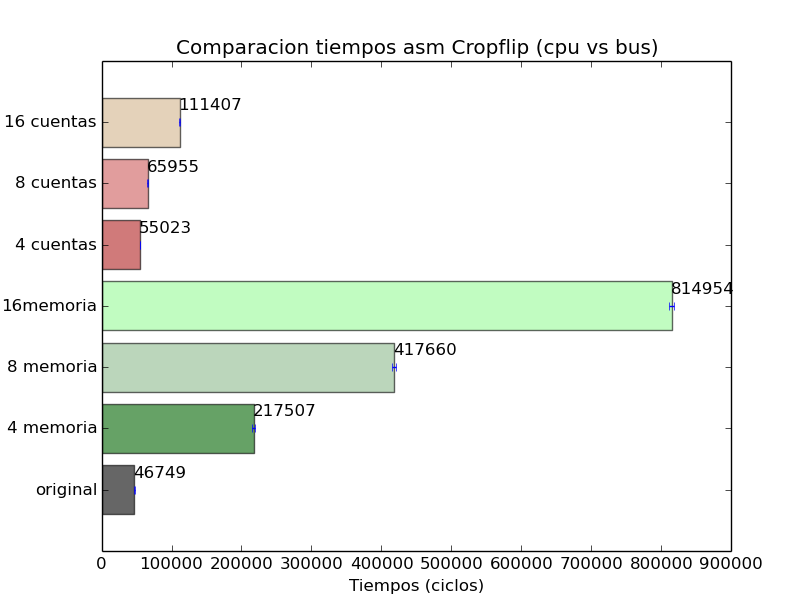
\includegraphics[width=350pt]{imagenes/cropCompC.png}

%En el gr\'{a}fico se nota la clara diferencia entre las corridas con optimizaciones y sin ellas. El criterio fue el mismo que aplicamos en los experimentos de m\'{a}s adelante (Haciendo 1000 iteraciones).

\newpage

\textbf{Experimento 1.3)}\\ \\ 
En este experimento consideraremos diferentes criterios realizando siempre 10 mediciones, con outliers, sin ellos, y agregando programas en C++ que trabajen en simult\'{a}neo.\\ \\

\noindent \textbf{a)}
Midiendo el Cropflip 10 veces los resultados fueron:\\ \\ 422861, 242136, 186857,\\ 194709, 234097, 221979,\\ 247912, 227976, 223245,\\ 200770.\\ 

\noindent\textbf{b)} Midiendo el Cropflip con programas en simultáneo los resultados fueron:\\ \\ 289209, 302654, 258757,\\ 254428, 248527, 254606,\\ 260391, 338981, 373612,\\ 280937 \\

\noindent \textbf{c)} \\ \textbf{10 mediciones}\\Esperanza: 240254.2 \\ Desv\'{i}o standard: 67250.78758 \\ Varianza: 4522668429.51111\\ 
\noindent \textbf{10 mediciones con el programa en simult\'{a}neo:}\\Esperanza: 286210.2 \\ Desv\'{i}o standard: 41607.01932 \\
Varianza: 1731144056.62222\\ 
\textbf{d)} \textbf{10 mediciones sin 2 outliers:}\\Esperanza: 224103 \\ Desv\'{i}o standard: 18595.78063 \\ Varianza: 345803057.14286\\ 

\noindent \textbf{e)} Analizamos las esperanzas y varianzas del filtro sin outliers, con outliers (La medición original) y con los otros programas simultáneos:\\
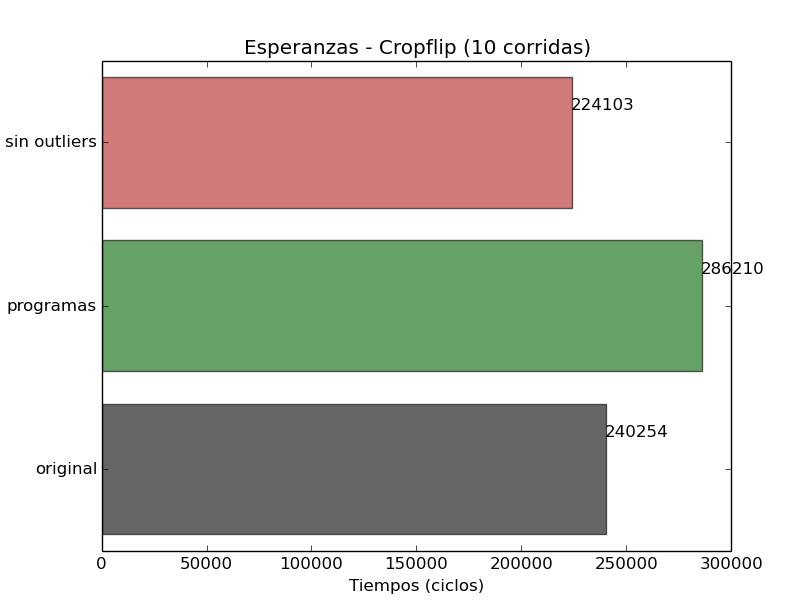
\includegraphics[width=300pt]{imagenes/esperanzas.png}

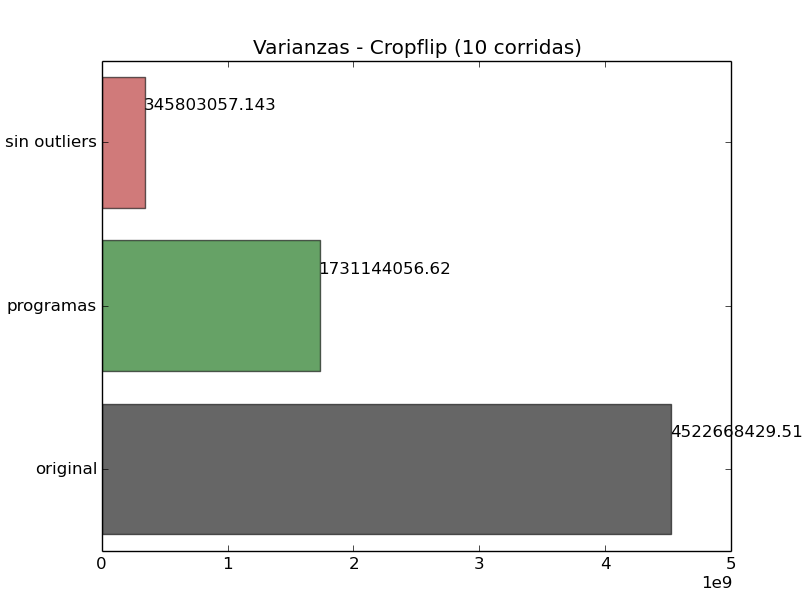
\includegraphics[width=300pt]{imagenes/varianzas.png}

Luego de observar estas mediciones hemos notado una varianza demasiado alta (y, en consecuencia, una falta de confiabilidad en las mediciones), por lo tanto, luego de probar con distintos m\'{e}todos de medici\'{o}n decidimos tomar el promedio de 1000 mediciones 10 veces, eliminar outliers y calcular luego nuevamente el promedio de las mediciones restantes. \\

\textbf{Experimento 1.4)}\\
Este experimento comparar\'{a} la performance de las implementaciones C y assembler que aplican el filtro cropflip (siguiendo el modelo de procesamiento secuencial y vectorial, respectivamente), probamos la implementaci\'{o}n en C con 4 distintos flags de optimizaci\'{o}n.

\begin{itemize}

\item \textbf{asm-} 46671 ciclos\\
\item \textbf{C O3-} 106740 ciclos\\
\item \textbf{C O2-} 106859 ciclos\\
\item \textbf{C O1-} 156148 ciclos\\
\item \textbf{C O0-} 613445 ciclos\\

\end{itemize}

NOTA: las l\'{i}neas peque\~nas azules en el tope de las barras representan el desv\'{i}o est\'{a}ndar del promedio de las mediciones que estamos mostrando.

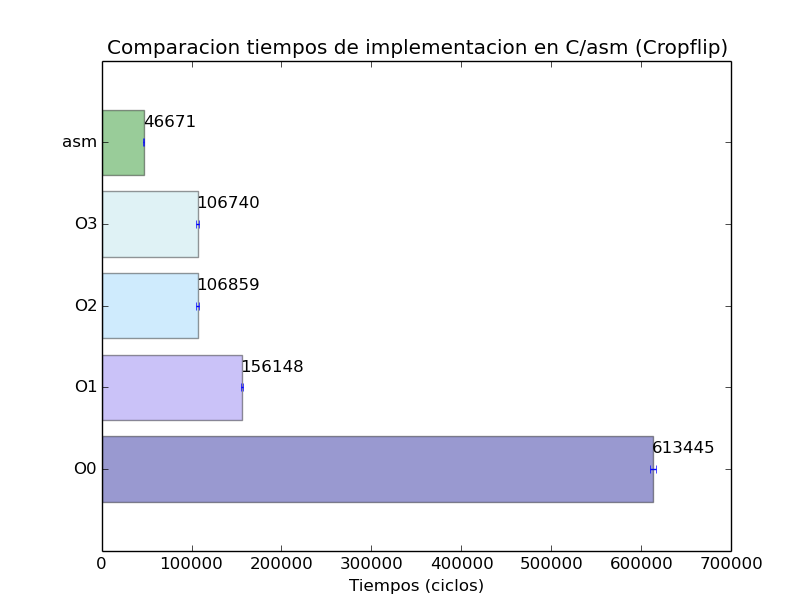
\includegraphics[width=300pt]{imagenes/CompCasm1.png}

Se observa en este experimento una notoria ventaja (en eficiencia temporal) del procesamiento vectorial de datos sobre el secuencial, incluso luego de haber aplicado las optimizaciones sobre el secuencial (que redujeron mucho el tiempo de procesamiento) la implementaci\'{o}n de assembler pudo aplicar el filtro mucho m\'{a}s r\'{a}pido y de manera m\'{a}s efectiva, mientras que entre las optimizaciones O2-O3 no hubo diferencia casi, indicando que no parece ser posible optimizar mucho m\'{a}s la implementaci\'{o}n en C debido a la limitaci\'{o}n que supone operar siguiendo una l\'{o}gica secuencial en casos en los que resulta mucho m\'{a}s ventajoso trabajar con varios datos al mismo tiempo.\\ \\ \\ \\

\textbf{Experimento 1.5) Cropflip - CPU vs bus de memoria}\\ \\
El experimento consistía en agregarle al filtro Cropflip en cada ciclo de la funci\'{o}n  4, 8 y 16 cuentas aritméticas, luego 4, 8 y 16 operaciones de memoria y ver como afecta cada una la performance. \\
Como la funci\'{o}n ejecuta pocas instrucciones en cada iteraci\'{o}n, con cualquier cosa que le añadimos se pudo ver una diferencia en la cantidad de ciclos de cpu que necesita para completarse. \\
Para cada test corrimos 10 veces 100 iteraciones del programa obteniendo 10 promedios de tiempo consumido, la funci\'{o}n original tarda aproximadamente 46 000 ciclos de procesador. Cuando insertamos 4 operaciones aritméticas el tiempo de procesamiento aumento a 55 000 ciclos aproximadamente, es decir, un 20\% mas. An\'{a}logamente, después de añadir 8 operaciones aritméticas, la cantidad de ciclos subi\'{o} a 65 000 aproximadamente, o sea un 41\%. Finalmente al agregar 16 operaciones aritméticas la funci\'{o}n tard\'{o} mas de lo esperado, 110 000 ciclos aproximadamente, lo que corresponde a un aumento del 139\% con respecto al filtro original. \\

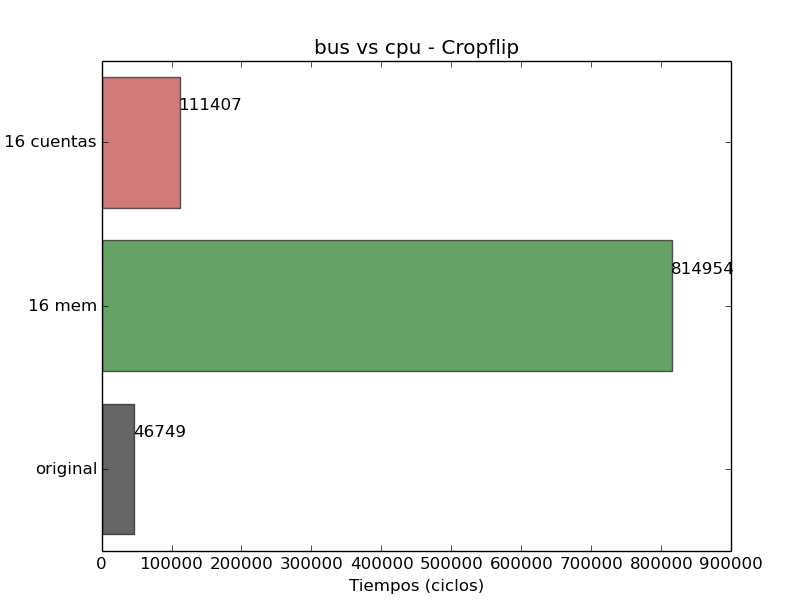
\includegraphics[width=300pt]{imagenes/bvmcrop.png}

En una primera impresi\'{o}n nos podríamos dejar engañar por los grandes números y porcentajes, sin embrago luego de lembrar que la funci\'{o}n cropflip_asm original no hace muchas operaciones, que el filtro itera 1 vez cada 4 píxeles (es decir 65536 veces), y que el procesador sobre el cual fueron hechas las pruebas genera 2 500 000 000 ciclos por segundo, podemos concluir que las cuentas aritméticas de enteros no generan un cuello de botella para el procesador. \\
A la hora de probar accesos a memoria la cosa fue muy distinta, cuando agregamos 4 el filtro necesit\'{o} aproximadamente 220 000 ciclos de reloj para terminar (Es decir un 378\% más). \\ Con 8 accesos a memoria mas comparado con la funci\'{o}n original, la cantidad de ciclos consumidos aumento a 417 000, generando así una suba del 807\%. \\ Aquí paramos un momento para remarcar algo: Al contrario de lo que esper\'{a}bamos, la cach\'{e} no pudo hacer que el porcentaje de incremento sea un poco menor a estrictamente lineal en funci\'{o}n a la cantidad de accesos a memoria agregados, de hecho con el doble de accesos a memoria el porcentaje de aumento fue mas que dos veces lo anterior. \\ Por \'{u}ltimo cuando probamos el filtro con 16 accesos a memoria los resultados fueron los siguientes, la función requirió de aproximadamente 815 000 ciclos de cpu para finalizar, esto implica una incre\'{i}ble suba del 1672\% (volvemos a notar que el porcentaje incrementado es mas del doble que el anterior). Luego de ver la suba que implico el agregado de accesos a memoria y después de realizar el mismo test con operaciones de tipo “mov” con registros e inmediatos y obtener casi los mismos resultados (incluso un poquito mejores) que con las operaciones aritméticas, podemos concluir que si bien el procesador es muy r\'{a}pido para distribuir datos que ya posee, la obtención de datos de la memoria implica un cuello de botella en el procesamiento del filtro, ya que esta acción tarda mucho mas que la mayoría de operaciones que no requieren datos que se encuentren fuera del procesador o de la instrucción. \\
Retomando el tema del orden de crecimiento de los tests, una posible teoría a este aumento “que no respeta la regla de 3 simple”, es que al usar en todas las mediciones los mismos 2 registros para todas las instrucciones extra, pudo haberse complicado la ejecución fuera de orden del procesador. Luego de notar esto volvimos a realizar las pruebas con mas diversidad de registros en las instrucciones aritméticas agregadas, y notamos un decremento en la tasa de aumento en relación a la cantidad de operaciones añadidas. \\ \\ \\ \\





\subsubsection{Sierpinski}

\textbf{Experimento 2.1) Sierpinski - secuencial vs vectorial}\\

Este experimento comparar\'{a} la performance de las implementaciones C y assembler que aplican el filtro sierpinski (siguiendo el modelo de procesamiento secuencial y vectorial, respectivamente), probamos la implementaci\'{o}n en C con 4 distintos flags de optimizaci\'{o}n.

\begin{itemize}


\item \textbf{asm-} 1618682 ciclos\\
\item \textbf{C O3-} 4114385  ciclos\\
\item \textbf{C O2-} 10599598 ciclos\\
\item \textbf{C O1-} 17026398 ciclos\\
\item \textbf{C O0-} 24125694 ciclos\\ \\ \\

\end{itemize}

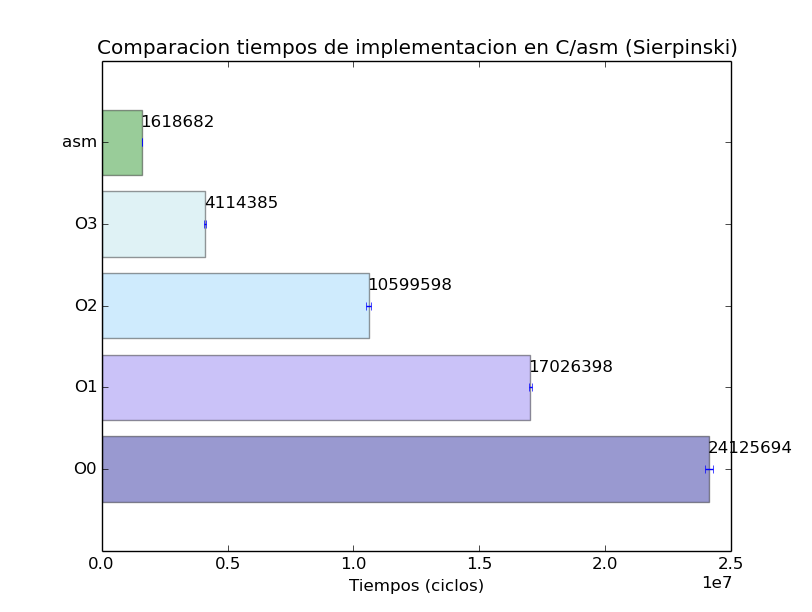
\includegraphics[width=350pt]{imagenes/CompCasm2.png}

En este experimento la ventaja de usar SIMD sigui\'{o} not\'{a}ndose con fuerza, mostrando una gran diferencia cuando es contrastado su tiempo de ejecuci\'{o}n con el de las distintas optimizaciones de la implementaci\'{o}n en C, si bien en este caso se not\'{o} que la optimizaci\'{o}n O3 tiene un gran impacto comparada con la O2, y lo mismo ocurri\'{o} al contrastar la O2 con la O1, y la O1 con la O0, suponemos que esto ocurre decido a que las optimizaciones del compilador son muy eficientes al trabajar sobre reducir el peso de operaciones aritm\'{e}ticas (operaciones de las que sierpinski se vale mucho para calcular el coeficiente).\\ \\ \\ \\

\textbf{Experimento 2.1) Sierpinski - CPU vs bus de memoria}\\ \\
Este experimento consiste en volver a realizar los tests del item 1.5 pero con la funci\'{o}n del filtro Sierpinski. Para realizarlo utilizamos la misma metodolog\'{i}a que empleamos al momento de realizar estas pruebas con Cropflip. La funci\'{o}n original que computa el filtro de este experimento arroja como resultado un uso de 1.62M ciclos de cpu (De ahora en adelante utilizamos la letra “M” para simbolizar millones y “K” para indicar miles). \\
Antes de empezar con los resultados podemos observar que la funci\'{o}n a evaluar realiza una cantidad notable mas de operaciones (muchas de ellas de punto flotante) en cada iteraci\'{o}n que la previamente testeada, por lo que esperamos obtener resultados diferentes, ya que agregar 4 instrucciones a un programa que posee 4 significa un aumento en la cantidad de operaciones del 100\%, sin embargo, añadirle la misma cantidad a una funcion que tiene 80 implica solo un aumento del 5\%. \\
Ahora s\'{i}, empecemos. Primero realizamos un \textit{benchmark} del filtro habi\'{e}ndole agregado 4 instrucciones aritmeteicas y la diferencia de performance fue inapreciable, en promedio solo 40K ciclos m\'{a}s que la original, o sea tan solo un 2.47\% mas. Luego probando con 8 operaciones aritmeticas vimos que la funci\'{o}n requiri\'{o}, en promedio, de 1.70M ciclos de cpu, es decir apenas un 4.94\% arriba del filtro original (exactamente el doble que lo anterior). \\ 
Por \'{u}ltimo hicimos el experimento agregando 16 instrucciones de la misma \'{i}ndole que las anteriores añadidas y el test arroj\'{o} un resultado de 1.84M de ciclos necesarios para completar la ejecuci\'{o}n, esto es un incremento del 13.58\%(Como en el item 1.5, no siempre el doble de operaciones insertadas implica el doble de crecimiento). Luego de realizar todos los tests aritmeticos podemos ver que este tipo de operaciones casi no afectan  la performance de la funci\'{o}n, luego observando que la misma posee igual cantidad de accesos a memoria que Cropflip, podemos concluir que la performance en promedio no se deteriora mucho luego de agregar instrucciones aritm\'{e}ticas de enteros por la gran cantidad de operaciones de punto flotante y SIMD que tiene el filtro. \\
Los experimentos con accesos a memoria fueron parecidos, cuando le agregamos 4 a la función esta aumentó su cantidad de ciclos a 1.64M, es decir, tan solo un 1\% más. Después añadimos 8 instrucciones de memoria al filtro original y el número de ciclos de CPU subió a 1.82M, esto implica una suba del 12\%, sorpresivamente 12 veces más que el anterior. Por último, con 16 operaciones de memoria la cantidad de ciclos consumidos fue de 2.10M, un 30\% más que el original. Notamos que el porcentaje de suba no era directamente proporcional con la cantidad de instrucciones agregadas. Nuestra hipótesis sobre este suceso es que como pusimos todas las operaciones extra juntas, el procesador no podia hacer ninguna otra instruccion mientras esperaba que le lleguen los datos de memoria. Para confirmar esta teoría volvimos a realizar el experimento esparciendo las operaciones de memoria entre las instrucciones aritmeticas de la funcion original, y el resultado fue positivo, en todas las pruebas el porcentaje de aumento varió entre 1\% y 2\%. \\ 
Finalmente podemos concluir que si bien las operaciones de memoria consumen muchos ciclos esperando los datos, el procesador es capaz de aprovechar ese tiempo realizando instrucciones aritmeticas entre ellas. \\

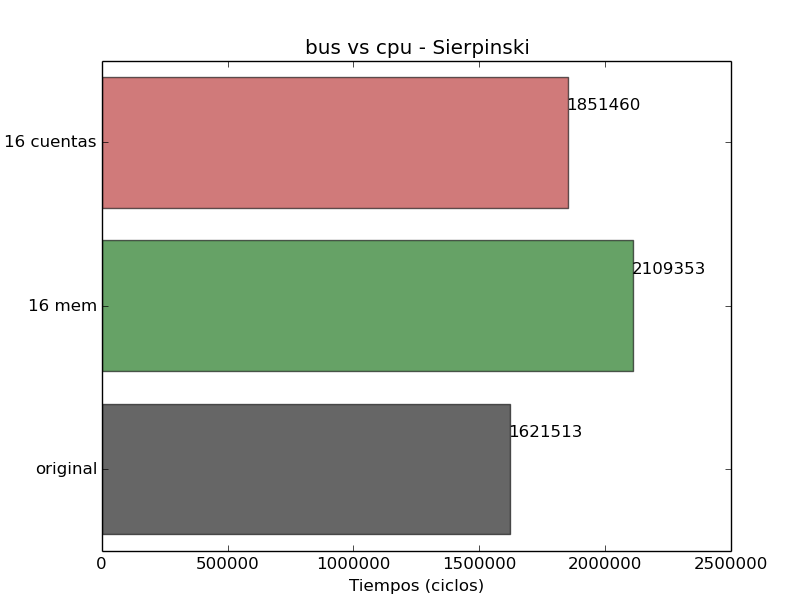
\includegraphics[width=300pt]{imagenes/bvmsierp.png}

\subsubsection{Bandas}

\textbf{Experimento 3.1) Bandas - saltos condicionales}

En este experimento corrimos el programa con el flag -O1, en comparaci\'{o}n con el mismo programa sin los condicionales. Como explicamos en el punto 1.2, -O1 ofrece ciertas optimizaciones del c\'{o}digo que reducen sustancialmente el 'branching', reemplaz\'{a}ndolo en lo posible por instrucciones aritm\'{e}ticas. Por ello, ya esper\'{a}bamos cierta diferencia a favor del programa sin condicionales. Sin embargo al correr los experimentos nos sorprendi\'{o} que la diferencia era abismal: El c\'{o}digo sin condicionales corre 3 veces m\'{a}s r\'{a}pido que el optimizado. Esto deja en evidencia lo ineficiente que es utilizar saltos condicionales, incluso si lo optimizamos.

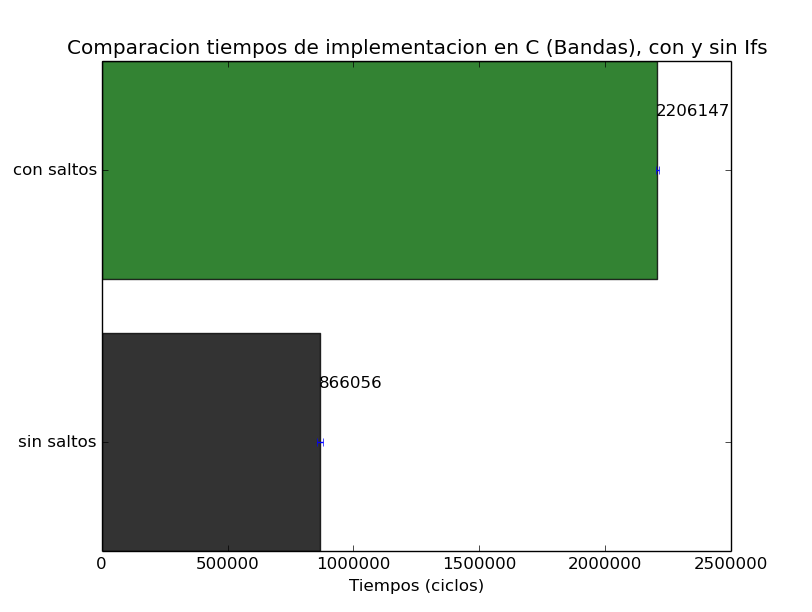
\includegraphics[width=350pt]{imagenes/cmpIFS.png}

\newpage

\textbf{Experimento 3.2) Bandas - secuencial vs vectorial}\\ \\

Este experimento comparar\'{a} la performance de las implementaciones C y assembler que aplican el filtro bandas (siguiendo el modelo de procesamiento secuencial y vectorial, respectivamente), probamos la implementaci\'{o}n en C con 4 distintos flags de optimizaci\'{o}n.

\begin{itemize}

\item \textbf{asm-}  516916 ciclos\\
\item \textbf{C O3-} 2205562 ciclos\\
\item \textbf{C O2-} 2165530 ciclos\\
\item \textbf{C O1-} 2214220 ciclos\\
\item \textbf{C O0-} 6931576 ciclos\\ \\ \\

\end{itemize}

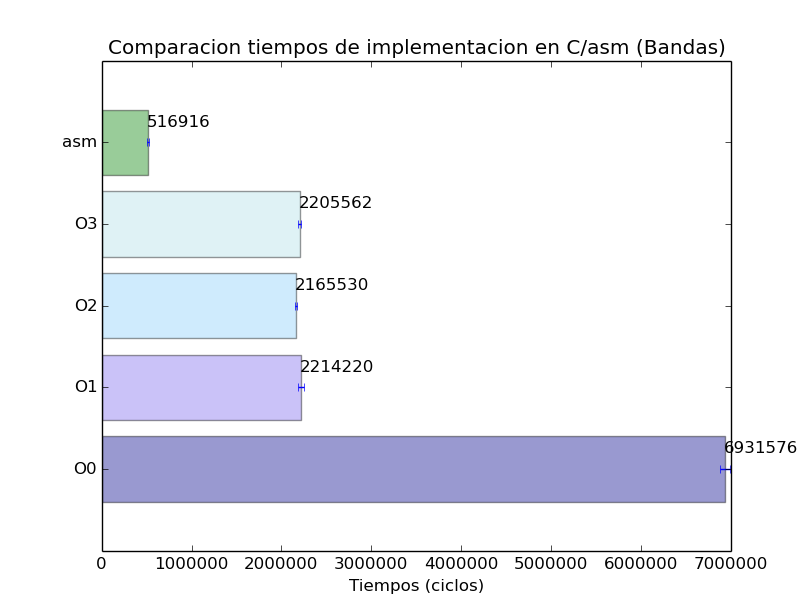
\includegraphics[width=350pt]{imagenes/CompCasm3.png}

Se puede notar en este gr\'{a}fico la ineficiencia de la implementaci\'{o}n en C, que es en parte remediada cuando se aplican las optimizaciones del compilador, si bien no se consigue obtener resultados cercanos al de la implementaci\'{o}n en assembler, ni avanzar mcuho m\'{a}s en las optimizaciones, ya que se ve c\'{o}mo luego del flag de optimizaci\'{o}n O1 las siguiente optimizacones parecen haberse estancado, quedando todas en el mismo nivel relativo (suponemos que el O3 supera en tiempo al O2 por poco debido a procesos que puede haber estado corriendo el sistema en el momento de tomar las mediciones, si bien se entiende que todas parecen estar en la misma l\'{i}nea aproximadamente), podr\'{i}amos arriesgarnos incluso a decir que no creemos que las optimizaciones con los siguientes flags (O4 en adelante) no har\'{a}n mucho m\'{a}s por mejorar la eficiencia temporal del procesamiento secuencial.

\newpage

\subsubsection{Motion Blur}

\textbf{Experimento 4.1) Motion Blur - secuencial vs vectorial}\\ \\

Este experimento comparar\'{a} la performance de las implementaciones C y assembler que aplican el filtro motion blur (siguiendo el modelo de procesamiento secuencial y vectorial, respectivamente), probamos la implementaci\'{o}n en C con 4 distintos flags de optimizaci\'{o}n.

\begin{itemize}

\item \textbf{asm-}  1577304 ciclos
\item \textbf{C O3-} 4698057 ciclos\\
\item \textbf{C O2-} 4889967 ciclos\\
\item \textbf{C O1-} 5513945 ciclos\\
\item \textbf{C O0-} 17694922 ciclos\\\\ \\ \\

\end{itemize}

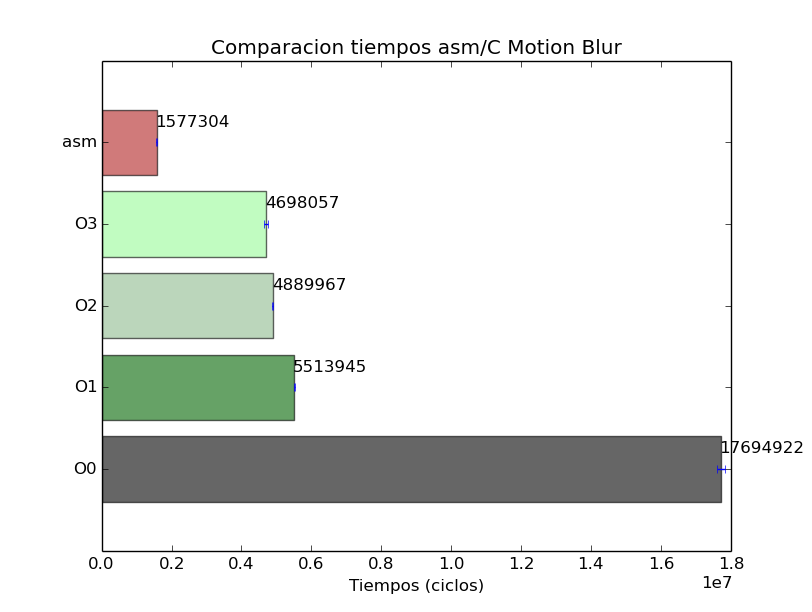
\includegraphics[width=350pt]{imagenes/CompCasm4.png}

En este experimento, nuevamente, la implementaci\'{o}n de assembler mostr\'{o} una clara diferencia (positiva) con las distintas optimizaciones de la de C, mientras que en C no se pudo optimizar el c\'{o}digo mucho m\'{a}s all\'{a} de la primera optimizaci\'{o}n, evidenciando una clara desventaja (nuevamente) de la implementaci\'{o}n en C en comparaci\'{o}n con la de assembler, lo que contribuye a afianzar la idea de que el procesamiento vectorial supera con mucho al secuencial (en los casos en que se pueden aprovechar sus ventajas).

\newpage

%\section{Enunciado y solucion} 
%\subsection{Filtro cropflip}

Programar el filtro \textit{cropflip} en lenguaje C y luego en ASM haciendo 
uso de las instrucciones vectoriales (\textbf{SSE}).

% ******************************************************************************
\vspace*{0.3cm} \noindent
\textbf{Experimento 1.1 - análisis el código generado}

En este experimento vamos a utilizar la herramienta \verb|objdump| para 
verificar como el compilador de C deja ensamblado el código C.

Ejecutar 
\begin{codesnippet}
\begin{verbatim}
objdump -Mintel -D cropflip_c.o
\end{verbatim}
\end{codesnippet}

¿Cómo es el código generado? 
Indicar
\begin{inparaenum}[\itshape a\upshape)]
    \item Por qué cree que hay otras funciones además de \verb|cropflip_c|
    \item Cómo se manipulan las variables locales
    \item Si le parece que ese código generado podría optimizarse
\end{inparaenum}

% ******************************************************************************
%\newpage
\vspace*{0.3cm} \noindent
\textbf{Experimento 1.2 - optimizaciones del compilador}

Compile el código de C con flags de optimización. Por ejemplo, pasando el flag 
\verb|-O1|\footnote{agregando este flag a \texttt{CCFLAGS64} en el makefile}. 
Indicar
\begin{inparaenum}
    \item Qué optimizaciones observa que realizó el compilador
    \item Qué otros flags de optimización brinda el compilador
    \item Los nombres de tres optimizaciones que realizan los compiladores.
\end{inparaenum}

% ------------------------------------------------------------------------------
% ------------------------------------------------------------------------------

\subsection{Mediciones}

Realizar una medición de performance \emph{rigurosa} es más difícil de lo 
que parece. 
En este experimento deberá realizar distintas mediciones de performance 
para verificar que sean buenas mediciones.

En un sistema ``ideal'' el proceso medido corre solo, sin ninguna 
interferencia de agentes externos. 
Sin embargo, una PC no es un sistema ideal. 
Nuestro proceso corre junto con decenas de otros, tanto de usuarios como 
del sistema operativo que compiten por el uso de la CPU. 
Esto implica que al realizar mediciones aparezcan ``ruidos'' o 
``interferencias'' que distorsionen los resultados.

El primer paso para tener una idea de si la medición es buena o no, 
es tomar varias muestras. 
Es decir, repetir la misma medición varias veces.
Luego de eso, es conveniente descartar los outliers
\footnote{en español, valor atípico: \url{http://es.wikipedia.org/wiki/Valor_atípico}}, 
que son los valores que más se alejan del promedio. 
Con los valores de las mediciones resultantes se puede calcular el promedio 
y también la varianza, que es algo similar el promedio de las distancias al 
promedio\footnote{en realidad, elevadas al cuadrado en vez de tomar el módulo}.

Las fórmulas para calcular el promedio $\mu$ y la varianza $\sigma^2$ son

$$
\mu = \frac{1}{n}\sum_{i=1}^{n} x_i \qquad \sigma^2 = \frac{\displaystyle\sum_{i=1}^{n}(x_i - \mu)^2} {n}
$$

% ******************************************************************************
\newpage
\vspace*{0.3cm} \noindent
\textbf{Experimento 1.3 - calidad de las mediciones}

\begin{enumerate}
    \item Medir el tiempo de ejecución de cropflip 10 veces. 
    \item Implementar un programa en C que no haga más que ciclar 
            infinitamente sumando 1 a una variable. 
            Lanzar este programa tantas veces como \emph{cores lógicos} tenga 
            su procesador. 
            Medir otras 10 veces mientras estos programas corren de fondo.
    \item Calcular el promedio y la varianza en ambos casos.
    \item Consideraremos outliers a los 2 mayores tiempos
     de ejecución de la medicion a) y también a los 2 menores,
     por lo que los descartaremos. Recalcular el promedio y la varianza después de hacer este descarte.
    \item Realizar un gráfico que presente estos dos últimos items.
\end{enumerate}

A partir de aquí todos los experimentos de mediciones deberán hacerse igual 
que en el presente ejercicio: tomando 10 mediciones, luego descartando 
outliers y finalmente calculando promedio y varianza.

% ******************************************************************************
%\newpage
\noindent\textbf{Experimento 1.4 - secuencial vs. vectorial}

En este experimento deberá realizar una medición de las diferencias de 
performance entre las versiones de C y ASM (el primero con -O0, -O1, -O2 y -O3) 
y graficar los resultados.

% ******************************************************************************
\vspace*{0.3cm} \noindent
\textbf{Experimento 1.5 - cpu vs. bus de memoria}

Se desea conocer cual es el mayor limitante a la
performance de este filtro en su versión ASM.

¿Cuál es el factor que limita la performance en este caso?
En caso de que el limitante fuera la intensidad de cómputo, entonces 
podrían agregarse instrucciones que realicen accesos a memoria extra y la
performance casi no debería sufrir. 
La inversa puede aplicarse, si el limitante es la cantidad de accesos a memoria.
\footnote{también podría pasar que estén más bien balanceados y que agregar
cualquier tipo de instrucción afecte sensiblemente la performance}
	
Realizar un experimento, agregando 4, 8 y 16 instrucciones aritméticas 
(por ej \verb|add rax, rbx|) analizando como varía el tiempo de ejecución.
Hacer lo mismo ahora con instrucciones de acceso a memoria, haciendo 
mitad lecturas y mitad escrituras (por ejemplo, agregando dos 
\verb|mov rax, [rsp]| y dos \verb|mov [rsp+8], rax|).\footnote{Notar que en el caso de acceder a \texttt{[rbp]} o \texttt{[rsp+8]} probablemente haya siempre hits en la cache, por lo que la medición no será de buena calidad. Si se le ocurre la manera, realizar accesos a otras direcciones alternativas.}
	
Realizar un único gráfico que compare:
\begin{inparaenum}
    \item La versión original
    \item Las versiones con más instrucciones aritméticas
    \item Las versiones com más accesos a memoria
\end{inparaenum}

Acompañar al gráfico con una tabla que indique los valores graficados.  
  
%\vspace*{0.3cm} \noindent
%\textbf{Experimento 1.6 (\textit{opcional}) - secuencial vs. vectorial (parte II)}
%
%
%Si vemos a los pixeles como una tira muy larga de
%bytes, este filtro en realidad no requiere \emph{casi}
%ningún procesamiento de datos en paralelo. Esto podría
%significar que la velocidad del filtro de C puede
%aumentarse hasta casi alcanzar la del de ASM. ¿ocurre esto?
%	
%Modificar el filtro para que en vez de acceder
%a los bytes de a uno a la vez se accedan como
%tiras de 64 bits y analizar la performance.

% ------------------------------------------------------------------------------
% ------------------------------------------------------------------------------

\subsection*{Filtro \textit{Sierpinski}}

Programar el filtro \textit{Sierpinski} en lenguaje C y en en ASM haciendo 
uso de las instrucciones vectoriales (\textbf{SSE}).

% ******************************************************************************
\vspace*{0.3cm} \noindent
\textbf{Experimento 2.1 - secuencial vs. vectorial}

Analizar cuales son las diferencias de performace entre las versiones de C 
y ASM de este filtro, de igual modo que para el experimento 1.4.

% ******************************************************************************
\vspace*{0.3cm} \noindent
\textbf{Experimento 2.1 - cpu vs. bus de memoria}

¿Cuál es el factor que limita la performance en este filtro?
Repetir el experimento 1.5 para este filtro.

\subsection*{Filtro \textit{Bandas}}

Programar el filtro \textit{Bandas} en lenguaje C y en en ASM haciendo uso de 
las instrucciones vectoriales (\textbf{SSE}).

% ******************************************************************************
\vspace*{0.3cm} \noindent
\textbf{Experimento 3.1 - saltos condicionales}

Se desea conocer que tanto impactan los saltos condicionales en el código 
de filtro Bandas con \verb|-O1| (la versión en C).\\
Para poder medir esto de manera aproximada, remover el código
que detecta a que banda pertenece cada pixel, dejando
sólo una banda.
Por más que la imagen resultante no sea correcta, será posible tomar una
medida aproximada del impacto de los saltos condicionales.
Analizar como varía la performance. 

% ******************************************************************************
\vspace*{0.3cm} \noindent
\textbf{Experimento 3.2 - secuencial vs. vectorial}

Repetir el experimento 1.4 para este filtro.

% ------------------------------------------------------------------------------
% ------------------------------------------------------------------------------

\subsection*{Filtro \textit{Motion Blur}}
Programar el filtro \textit{mblur} en lenguaje C y en ASM haciendo uso de 
las instrucciones \textbf{SSE}.

% ******************************************************************************
\vspace*{0.3cm} \noindent
\textbf{Experimento 4.1}

Repetir el experimento 1.4 para este filtro


\section{Conclusiones}
\textbf{C y sus optimizaciones vs ASM} \\
Luego de realizar este Trabajo Práctico podemos concluir con total certeza que, en cuanto a tiempos de ejecución, \textit{Assembler} supera ampliamente a C; y queda en evidencia que, cuanto más cerca se trabaja del código máquina, más óptimo es el resultado. \\
En cuanto a las optimizaciones, queda claro que C presenta muchos mejores tiempos optimizado que sin optimizar; aunque en algunos casos no se notan grandes diferencias entre O1, O2 y O3 (Incluso llegamos a ver casos en donde O3 estaba en el mismo nivel que O2). \\
Nuestra conclusión al respecto es que, a pesar de que \textit{ASM} pierde la claridad y el parecido con el lenguaje \textit{"humano"} que puede llegar a tener C, vale la pena conocer los grandes beneficios que tiene programar en el más bajo nivel. \\
También esto nos genera curiosidad de que tan poco eficientes serán lenguajes de más alto nivel, ya que sacrifican optimizaciones que se podr\'{i}an aplicar a c\'{o}digos (desechando procesos que sabemos que no vamos a necesitar en un programa en particular, por ejemplo) y se pierde versatilidad para poder proveer al programador un entorno m\'{a}s amigable y f\'{a}cil de asimilar. \\
Esto se deber\'{i}a a que en un punto, al proveer instrucciones de alto nivel que encompasan varias instrucciones de un lenguaje de m\'{a}s bajo nivel, estamos dejando de lado todas las infinitas combinaciones de instrucciones que se podr\'{i}an utilizar para ejecutar programas de manera distinta, es decir que limitamos las opciones para resolver un determinado problema que tenemos a unas pocas combinaciones de instrucciones determinadas por el lenguaje de alto nivel. \\

\textbf{Optimizaciones en el ASM} \\
Luego de programar durante la carrera utilizando variables y condicionales de forma constante y sin pensarlo dos veces, nos encontramos con ciertas realidades bastante duras: Los accesos a memoria y el \textit{branching} son \textbf{altamente ineficientes}. Como vimos previamente (Ver experimentos \textbf{1.5} y \textbf{2.1}), agregar operaciones aritméticas empeoran el tiempo de ejecución, pero los accesos a memoria son extremadamente peores si no son amortiguados como vimos en el experimento \textbf{2.1}. Esto nos sirvió bastante para ver por nosotros mismos lo que nos enseñan en teoría desde Organización del Computador 1: La memoria \textbf{es realmente lenta} en comparación a los registros del CPU. \\
En cuanto al \textit{branching}, lo tuvimos que comprobar por nosotros mismos (Ver implementación del Bandas en \textbf{2.1.3}): La utilización de saltos condicionales no parece ser gran problema en C, pero en ASM se nota la gran diferencia de performance y claridad en el código. Como ya vimos en el experimento \textbf{3.1}, por más que se optimice con O1 (Que reduce la ineficiencia de los saltos condicionales), el código sin saltos tarda tres veces menos que el optimizado. \\


\textbf{Conclusiones personales} \\
La idea de este Trabajo Práctico era expandir nuestros conocimientos de \textit{Assembler} adquiridos en el \textbf{TP1}, entendiendo como funciona SIMD y de qué manera se puede programar manejando varios datos al mismo tiempo. A su vez, aprendimos a medir en tiempo real nuestros propios programas por primera vez en la carrera, y eso nos empujó a querer superar nuestro propio código varias veces: Una vez que tuvimos terminados los cuatro filtros comenzamos a optimizarlos, mirando la cantidad aproximada de ciclos que tardaban, y pensando de qué manera se podría llegar a un mejor resultado. \\
Gracias a ese desafío, comprendimos la potencia de algunas instrucciones tales como \textit{pshuf} (Que nos terminó ahorrando varias líneas de código), y aprendimos nuevas maneras de pensar los problemas, como aprovechar el uso de \textit{máscaras} (Que terminó siendo más limpio, claro y rápido que cualquier otra forma de encarar el filtro \textbf{Bandas}). \\
También ganamos una nueva perspectiva en cuanto a la programación en C, conociendo sus optimizaciones y sus debilidades en cuanto a eficiencia.
Incluso, conversando con docentes, supimos que aún se puede llevar el asunto a otro nivel, con el uso de herramientas m\'{a}s avanzadas, como el \textit{multithreading}.

\end{document}


